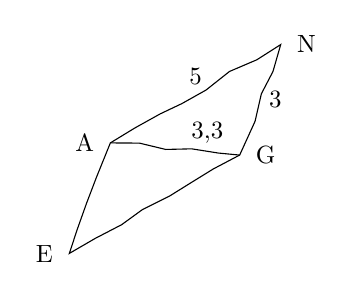
\begin{tikzpicture}[rotate=30,every node/.style={scale=0.9},scale=0.5]

\coordinate (A) at (0,0);
\coordinate (N) at (5,0);
\coordinate (G) at (2.69,-1.91);
\coordinate (E) at (-2.31,-1.91);

\draw[decorate,decoration={random steps,amplitude=1pt,segment length=10pt}] (A) node [left=3pt]{A}--(N) node [right=3pt]{N}--(G) node [right=3pt] {G}--(E) node [left=3pt] {E}--cycle;
\draw [decorate,decoration={random steps,amplitude=1pt,segment length=10pt}] (A)--(G);
\path (A)--(N) node[midway,above]{5};
\path (N)--(G) node[midway,right]{3};
\path (A)--(G) node[near end,above]{3,3};

\end{tikzpicture}